\documentclass[preprint,12pt]{elsarticle}
%\documentclass[preprint,12pt]{article}
\usepackage{graphicx}
\usepackage[margin=1.0in]{geometry}
\usepackage{color, colortbl}
\usepackage{hyperref}
\usepackage{float}
\usepackage{lineno}

%\linenumbers
% \usepackage[affil-it]{authblk}
\usepackage{subcaption}
\newcommand{\note}[1]{\textcolor{blue}{#1}}
\definecolor{LightCyan}{rgb}{0.88,1,1}
\definecolor{LightRose}{rgb}{1,0.88,0.88}
\definecolor{LightGreen}{rgb}{0.88,1,0.88}

\title{Data Compression using Auto-Encoders for CLAS12 Online}
\author[1]{Gagik Gavalian}

\address[1]{Jefferson Lab, Newport News, VA, USA}
%\address[2]{CRTC, Department of Computer Science, Old Dominion University, Norfolk, VA, USA}


\begin{document}

%\begin{titlepage}
\begin{abstract}
In this article, we present the results of using Auto-Encoders for compressing the pulse data from CLAS12 detector systems.
The raw pulse form from Analog to Digital Convertors (ADC) is compressed to decrease raw data size. The results show that the pulses
can be compressed by a factor of 4, without significant loss in the pulse integral (about $1.4\%$).
\end{abstract}
%\end{titlepage}
\maketitle


\section{Introduction}

During past few years there was a big interest in using Artificial Intelligence (AI) in 
various ares of nuclear physics, from data processing to physics analysis. With continuously 
improving methods of Machine Learning (ML) and computational hardware it becomes easy to 
substitute some computational tasks with ML algorithms leading to smaller and computationally
more efficient code base. In this article we discuss implementation of Convolutional Auto-Encoders 
for de-noising data from CLAS12~\cite{Burkert:2020akg} tracking detectors (Drift 
Chambers~\cite{Mestayer:2020saf}). The de-nosing was used to analyze simulated data to measure
improvement on track reconstruction efficiency.

\section{Motivation}
\label{section-motivation}

%Data stored from physics experiments consists of "events" that record information from a setup for one interaction of the incident beam particle
%with the target. These "events" are processed independently to identify particles and tracks identified by different detector components and construct a physics event, which is then used for high-level physics analysis. The information stored in one "event" is a collection of responses from all detector components with unique data structures. The data collected during the experiment undergoes several transformations before it reaches the stage where it is used for physics analysis.

Physics experiment data consists of "events," each representing information captured from a single interaction between an incident beam particle and the target. These events are processed individually to identify particles and reconstruct tracks using data from various detector components. This process builds a complete physics event, which serves as the foundation for high-level physics analysis. Each event encapsulates a collection of responses from all detector components, organized in unique data structures. Before reaching the stage of physics analysis, the collected data undergoes multiple transformations to prepare and refine it for further study.

\begin{itemize}
\item The data acquisition records data from all detector components for one instance of interaction in raw format  (usually times and accumulated charge in each component of each detector system) 
\item In the next stage, the raw data is transformed from its digital form to values with units, such as time in milliseconds and energy in eV.
\item The reconstruction program analyses data from each detector to identify related signals and combines signals from various detectors to identify particles in each event (collision instance). The produced output contains tables with information about the particles in the event and the responses of each particle in each detector component, helping to identify particle species.
\item For each physics analysis, different sets of selection algorithms are used to identify the physics reaction in each event and physics observables are calculated based on detected particles in the event, and the output is produced containing a columnar table for final physics analysis. 
\end{itemize}

In traditional CLAS~\cite{CLAS:2003umf} experiments, different data formats were used at each stage of the data lifecycle, leading to unnecessary complexity. This required supporting multiple file formats and maintaining numerous conversion tools. Additionally, users developed dozens of data selection and filtering tools tailored to specific formats, all of which required ongoing maintenance. Initially, a similar approach was considered for the CLAS12~\cite{Burkert:2020akg} experiment during its early software development stages.

However, experienced developers quickly recognized the challenges of this approach and envisioned a more streamlined solution. To address these issues, it was decided to adopt a single data format for all stages of the experimental data lifecycle. Several existing formats, such as ROOT~\cite{Brun:1997pa}, LCIO~\cite{Aplin:2012kj}, and HDF5~\cite{HDF5:2000pa}, were evaluated. While each had its strengths, none were found to efficiently support all stages of data transformation. Furthermore, the growing diversity of data analysis frameworks and programming languages introduced additional challenges, as seamless integration required appropriate language bindings—complicating the use of existing formats in unified workflows.

To overcome these limitations, the High-Performance Output (HiPO)~\cite{hipo5p0:2025jk} data format was developed specifically for CLAS12. HiPO is designed to efficiently handle all stages of experimental data processing, from reconstruction workflows to final columnar data analysis. It also provides language bindings for a variety of programming languages used within the collaboration, including C++, FORTRAN, Python, Java, and Julia, ensuring broad compatibility and streamlined workflows.


To ensure usability across all workflows of data processing, several key requirements were established for the data format:

%Several requirements were imposed to ensure usability in all workflows of data processing, as follows:
\begin{itemize}
\item {\bf Serializable:} The CLAS12 reconstruction workflow follows a Service-Oriented Architecture (SOA) that operates on a heterogeneous platform using message passing. The data format was designed to be easily serializable, enabling efficient transmission of event data to individual reconstruction services.
\item {\bf Compression Efficiency:} To minimize storage demands, the data format incorporates compression. The compression algorithm must balance speed and compression ratio, as high compression speed is critical for managing the large data volumes produced by experimental setups, particularly in high-rate nuclear physics experiments where maintaining high data throughput is essential.
\item {\bf Random Access Capability:} The format must support random access to specific data collections within a file. This functionality is vital for debugging, selectively writing subsets of data, and supporting multi-threaded applications that process data chunks asynchronously.
\item {\bf Data Grouping Functionality:} The format should enable the grouping of related datasets, allowing for efficient tagging or marking of different datasets. This capability facilitates the targeted reading of specific groups without requiring the processing of the entire dataset.
\end{itemize}

The reconstruction of experimental data in CLAS12 is written in Java, for this reason, Java is the primary development platform of the HiPO library, and the C++ library is developed in parallel, sometimes lagging in features, but they are being slowly ported to the C++ code. Most of the example codes in this article are Java, the equivalent C++ examples can be found in the repository.
There are experimental bindings to Python and Julia, which are not actively developed due to limited use by collaborators.
The subsequent chapters will explore the features of the HiPO data format in greater detail, with illustrative examples.

\section{Studies with simulated data}

\subsection{Single Pulse Simulations}

The studies with the network were first conducted on simulated data to fine-tune the network before studying the impact on real data.
Pulses were generated using a Landau function on top of a flat background. 
\begin{equation}
L(x)=e^{-\frac{1}{2}(\frac{x-x_0}{\sigma} + e^{\frac{x-x_0}{\sigma}}) }
%(\frac{x-x_0}{$sigma} + e^{\frac{x-x_0}{$sigma}}})
\end{equation}

For each sample the position of the peak ($x_0$) was generated using a pseudo-random generator and the sigma value of 0.015 was used (which is similar to the pulses we see from the detectors).
A large training sample was used to train the autoencoder and a validation sample (also randomly generated) was used to compare the output from the network to the original pulse shape. For our initial studies, the network architecture [48,24,12,24,48] was used with {\bf ReLU} activation functions for hidden layers and {\bf Linear} activation function for the output layer.
The results are shown in Figure~\ref{fig:results_sp_48}. 

\begin{figure}[h!]
\centering
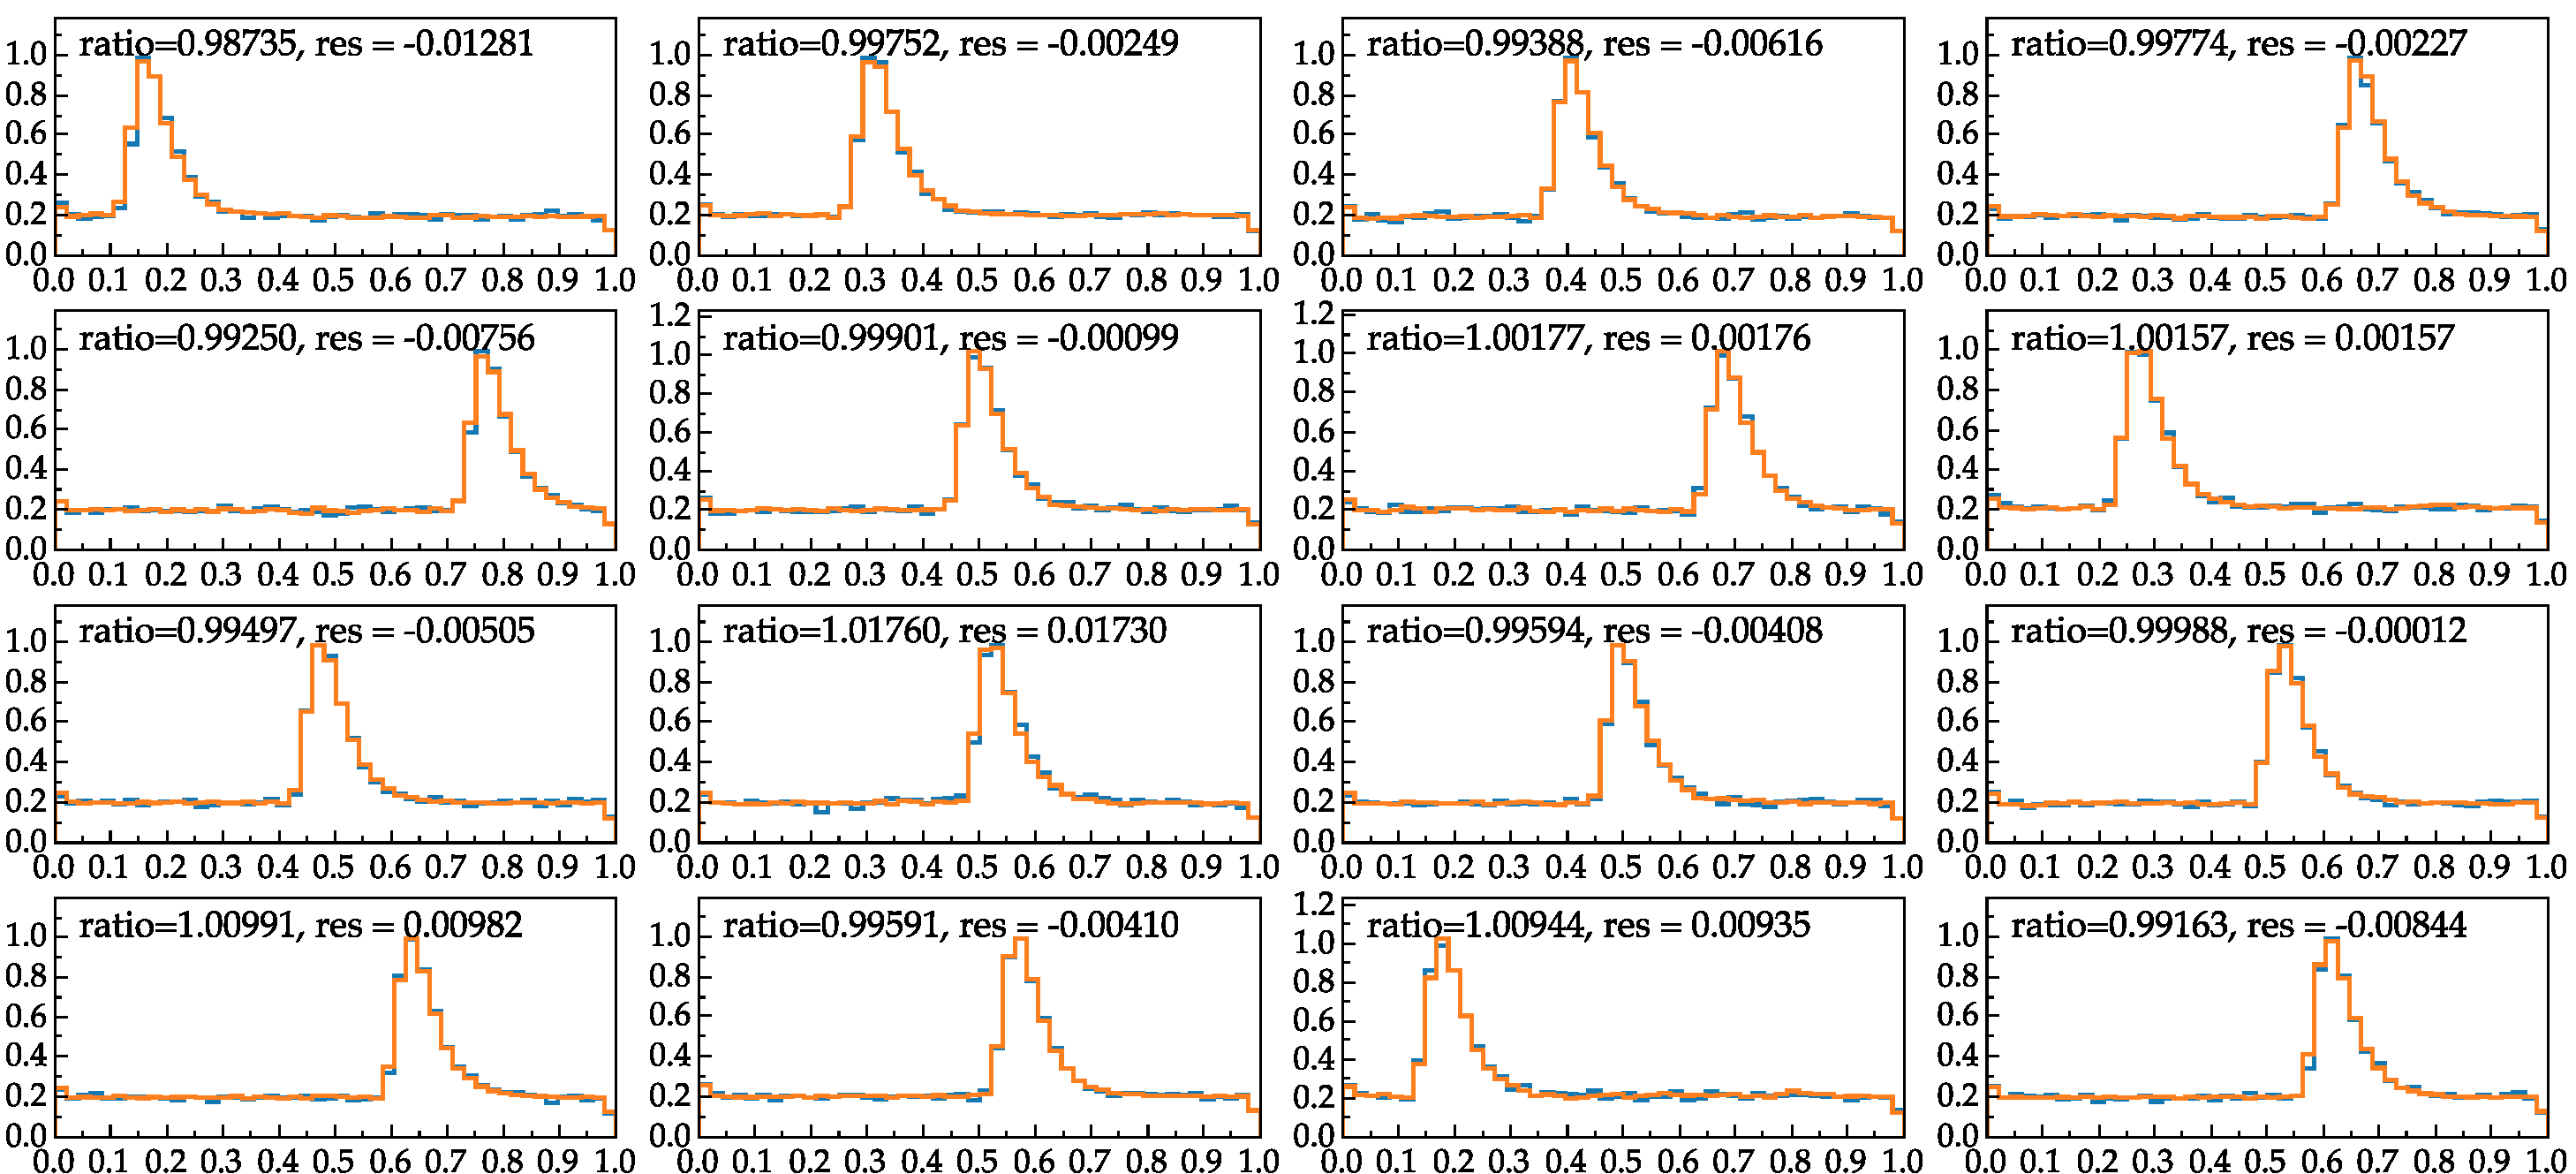
\includegraphics[width=0.9\columnwidth]{results_sp_48.pdf}
\caption{Original pulses plotted with reconstructed pulses overlayed. The data is produced by simulating a single pulse in the 48-bin region.} 
\label{fig:results_sp_48}
\end{figure}

It can be seen from the figure that the decoder reconstructs the pulses from encoded data with great accuracy, and the stored data is 4 times smaller (vector of the length 12 for the middle layer).
In Figure~\ref{fig:results_sp_48_res} (left) the distribution of the normalized difference of the pulse integral is plotted for the validation sample. As can be seen from the figure the reconstructed from the encoding pulse integral is on average in agreement with the input pulse with a resolution of about $0.7\%$. In Figure~\ref{fig:results_sp_48_res} (right) the time difference is calculated for the original pulse and the decompressed pulse. The time is calculated assuming that the 48 bins in the pulse represent a timing window of $48~ns$, the resulting difference is multiplied by $1000$ and the difference is given in pico-seconds.

\begin{figure}[h!]
\centering
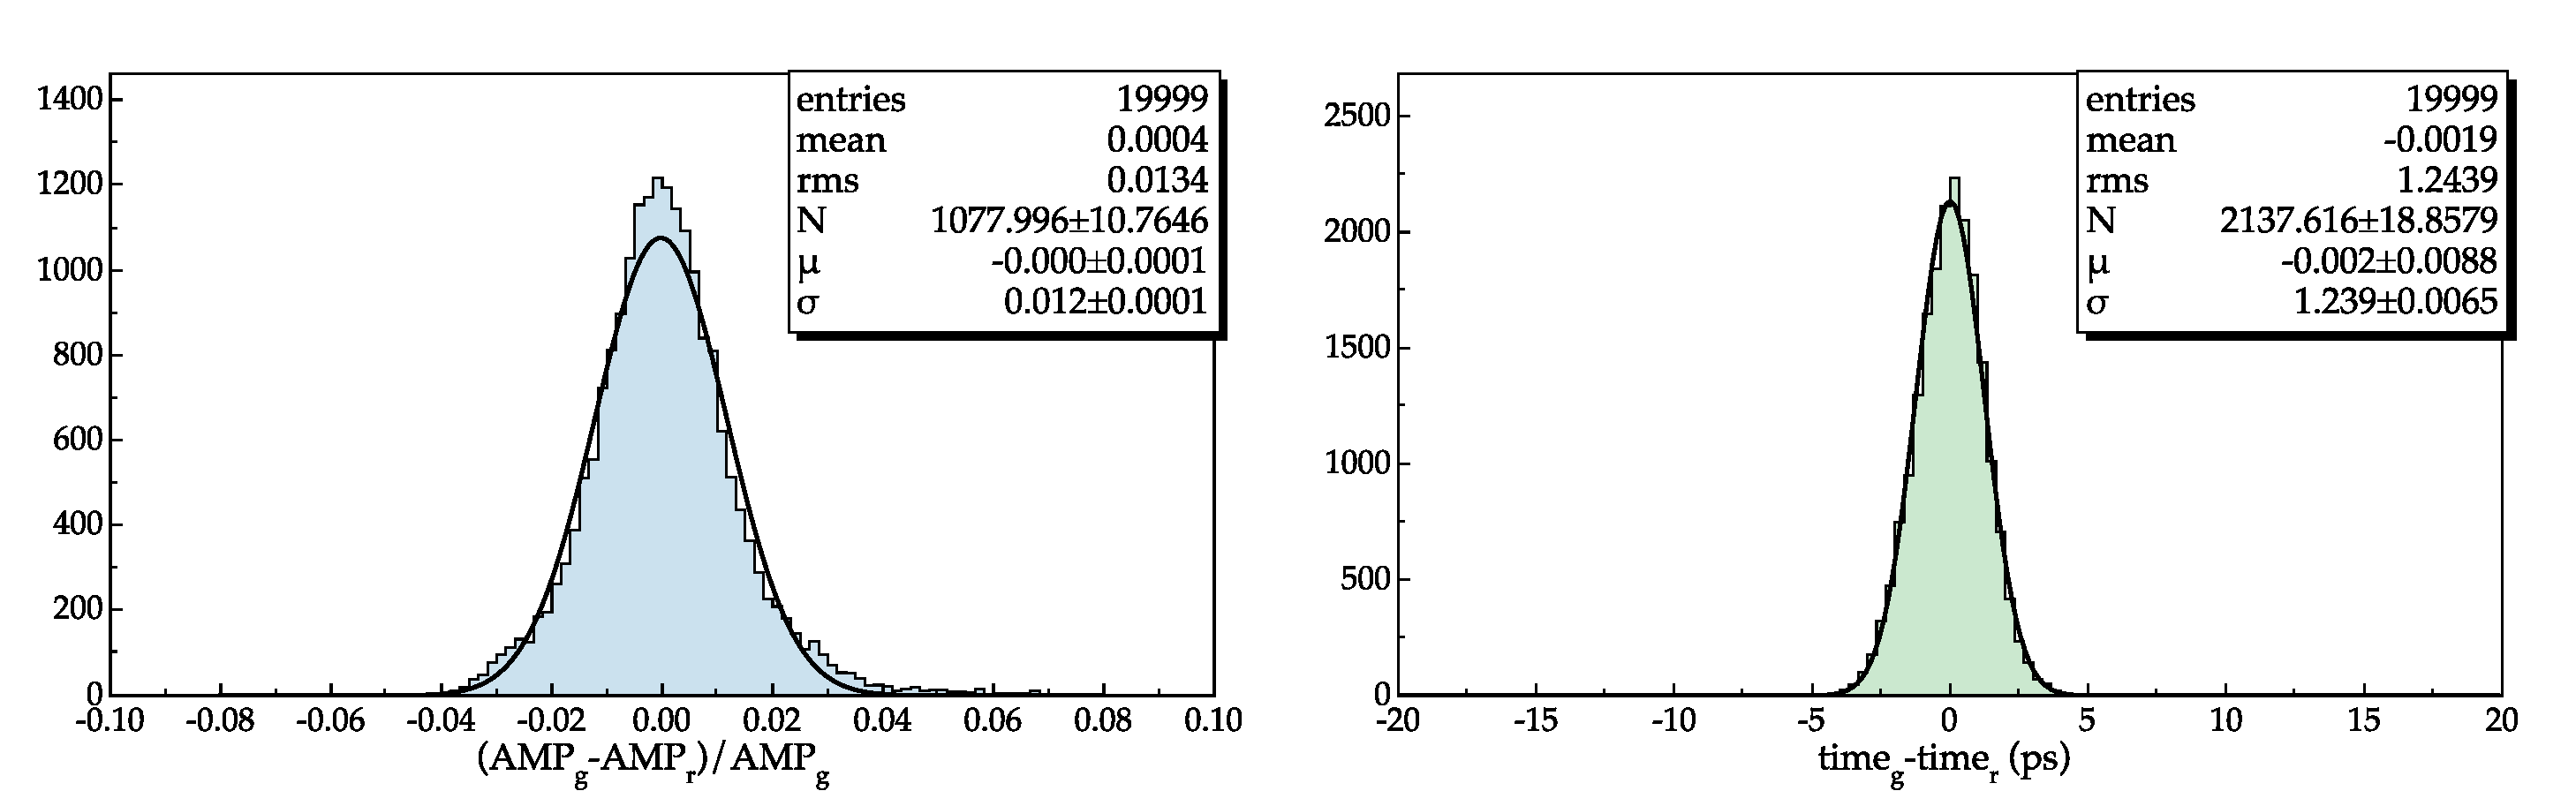
\includegraphics[width=0.9\columnwidth]{out_evaluate_csv_single_24.pdf}
\caption{The resolution of the pulse integrals. The integral of the pulse is compared to the integral calculated from decompressed pulses (on the right), and time calculated from the original pulse is compared to the time calculated from the decompressed pulse.} 
\label{fig:results_sp_48_res}
\end{figure}

In real experimental conditions, it is not uncommon to have two pulses in a given time window when the electronics are being read. Our next study is to use the same network architecture for training a network for compressing two pulse inputs.

\subsection{Double Pulse Simulations}

To study the compression of double pulse data we generated a new sample consisting of two pulses with random mean positions and random height ratios, the width of the pulse was kept the same (with $\sigma=0.015$). The results of compression and decompression for two pulse data are shown in Figure~\ref{fig:results_dp_48}. It can be seen from the figure that the network is able to accurately reconstruct the peak positions but in some cases, the heights and the widths of the peaks do not match the input peak, which leads to degraded accuracy for peak integral calculations. 

\begin{figure}[h!]
\centering
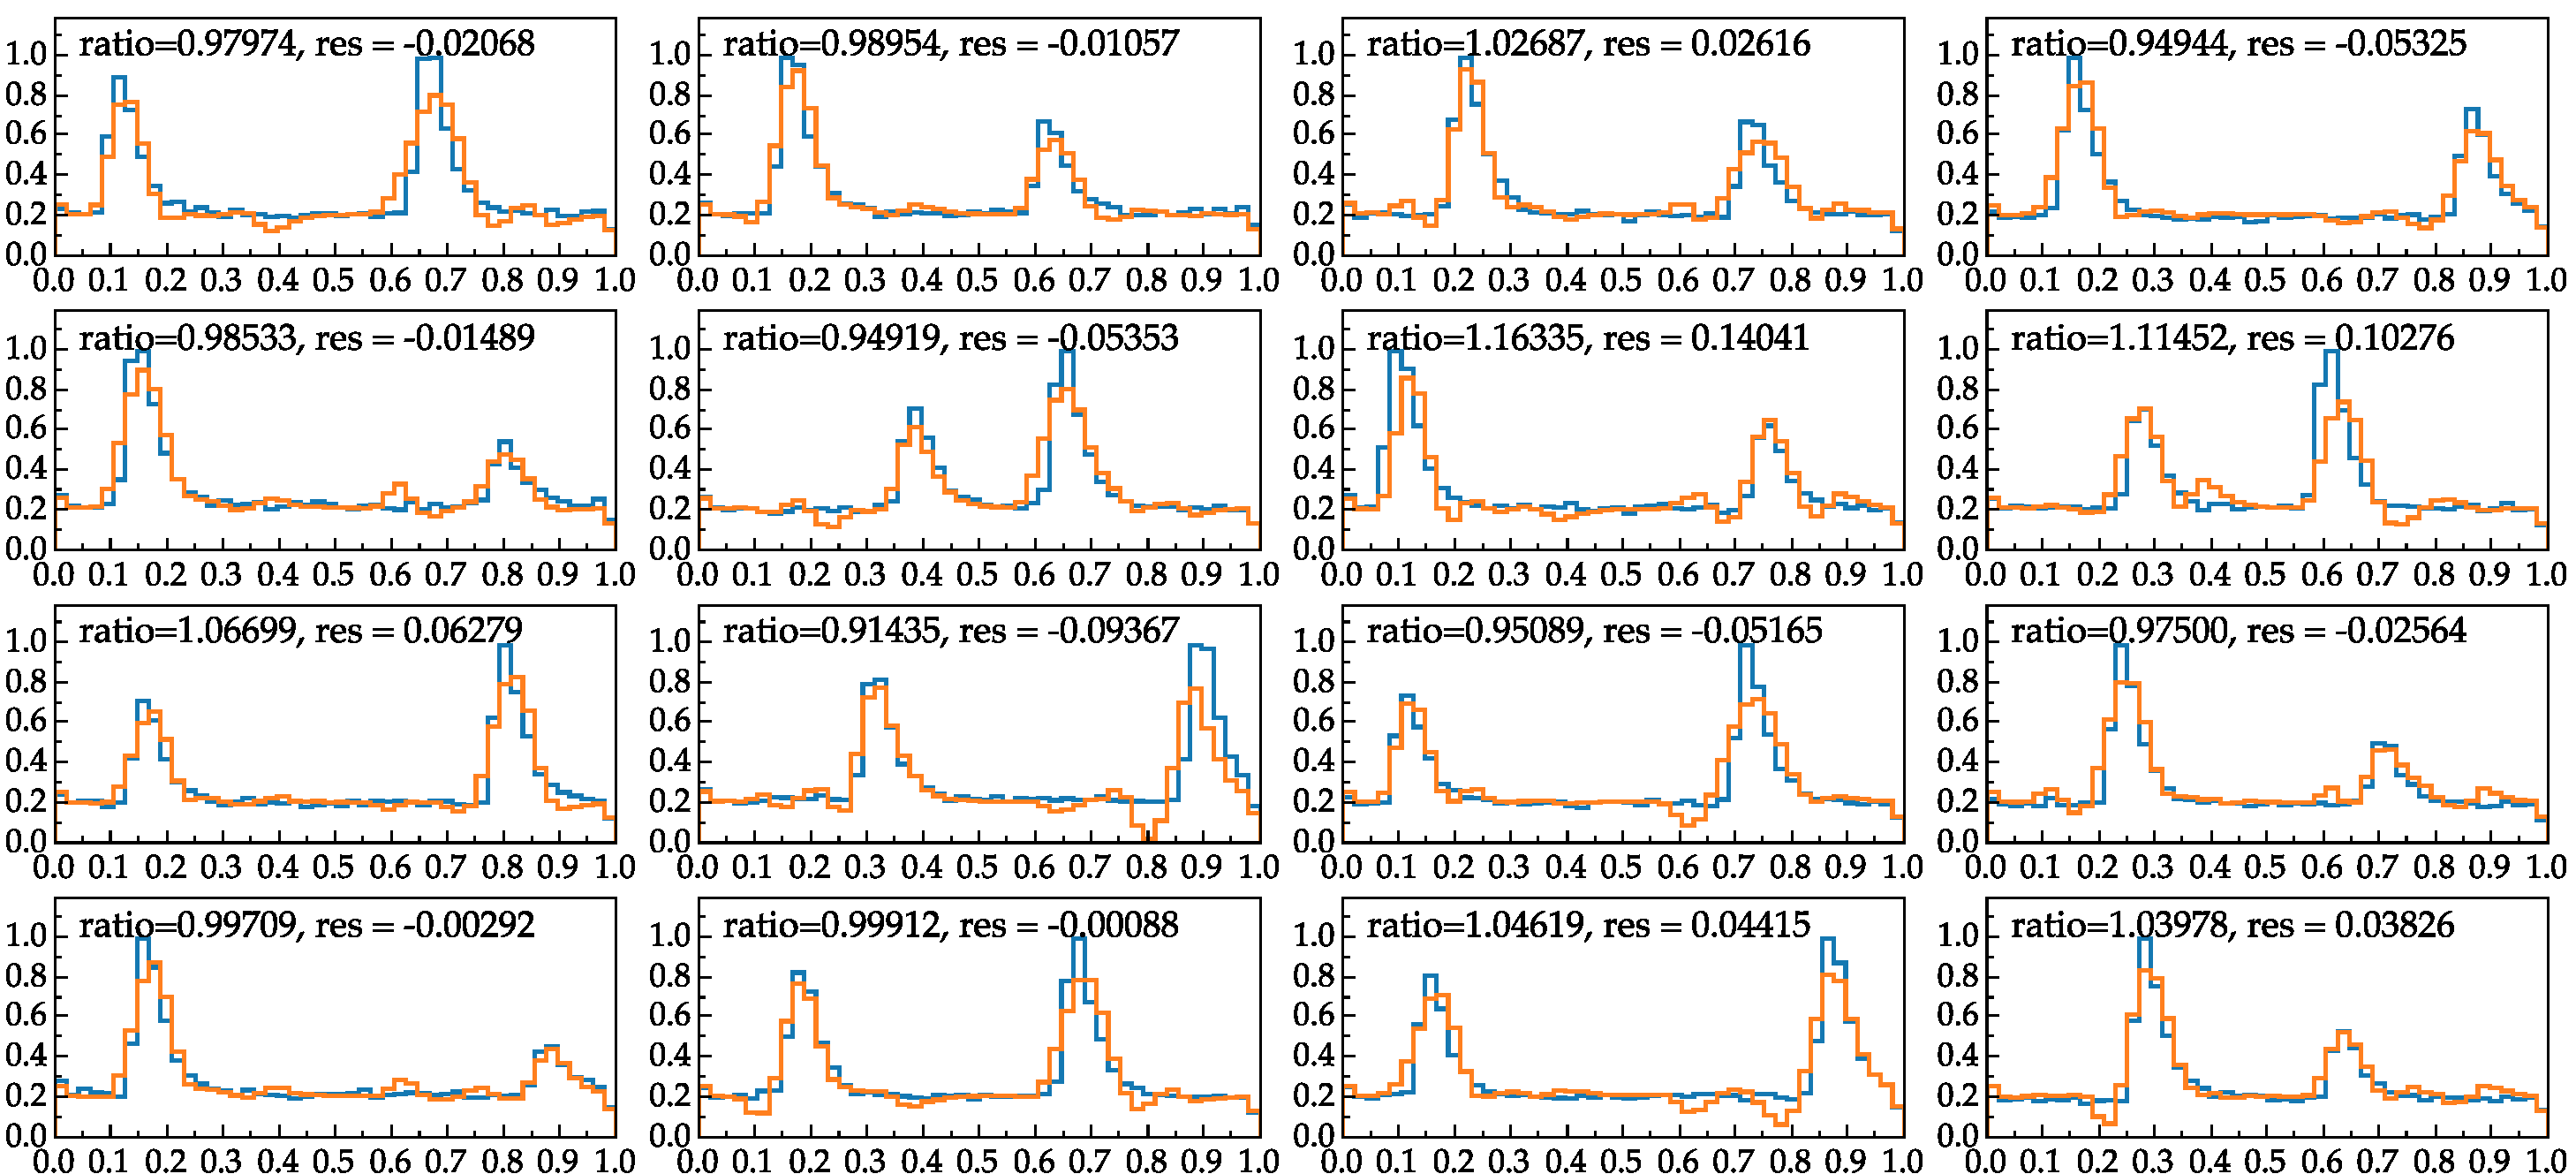
\includegraphics[width=0.9\columnwidth]{results_dp_48.pdf}
\caption{Generated double pulses plotted with the decompressed pulses overlayed. The compression is done with the original auto-encoder [48,24,24,12,24,24,48] architecture. The data is produced by simulating a single pulse in the 48-bin region.} 
\label{fig:results_dp_48}
\end{figure}

The average resolution for the peak integral reconstruction is shown in Figure~\ref{fig:results_dp_48_res}, and is about $4\%$. It's worth mentioning that the heights of the peaks being reconstructed with degraded accuracy can lead to inaccurate pulse timing calculations.

\begin{figure}[h!]
\centering
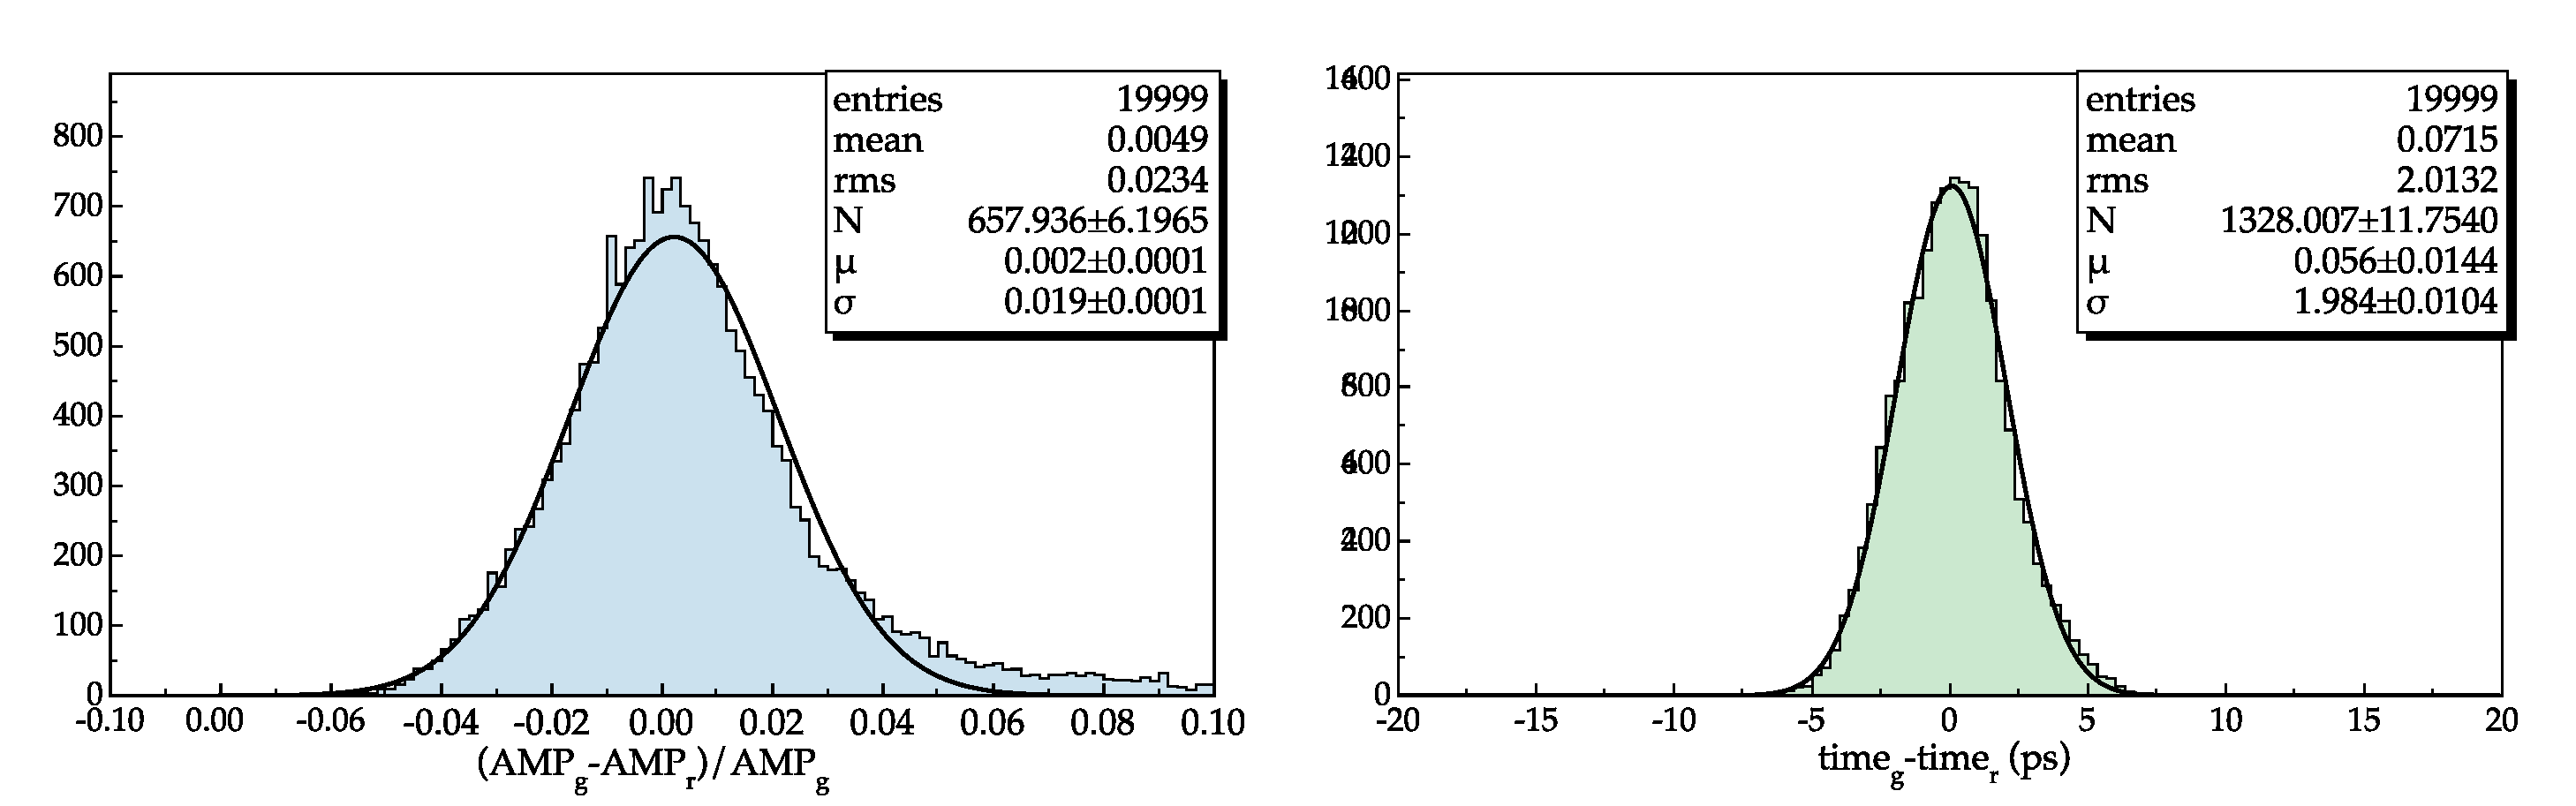
\includegraphics[width=0.9\columnwidth]{out_evaluate_csv_double_24.pdf}
\caption{The resolution of the pulse integrals (double pulses). The integral of the pulse is compared to the integral calculated from decompressed pulses (on the right), and the time calculated from the original pulse is compared to the time calculated from the decompressed pulse.} 
\label{fig:results_dp_48_res}
\end{figure}

To improve the two-pulse data compression a different network architecture was considered. Traditionally the autoencoders are constructed in a way that each subsequent layer starting from the input layer is smaller in size. This can potentially cause some issues when the input vector is not large enough, where the subsequent layer already has to find a more compact representation of the input. 
Following the logic from convolutional networks, one would expect that the layer following the input layer should be larger to be able to encode some different features from the input vector into much larger space, before trying to compress it. Inspired by this logic the network architecture was changed to have a larger hidden layer to follow the input layer in the network and changed the architecture to 
{\bf [48,96,48,24,12,24,48,96,48] }, while keeping it symmetric for both the encoder and decoder sides. The new network was trained on the same training sample with double pulses from our previous test, and the results can be seen in Figure~\ref{results_dp_96.pdf}. 

\begin{figure}[h!]
\centering
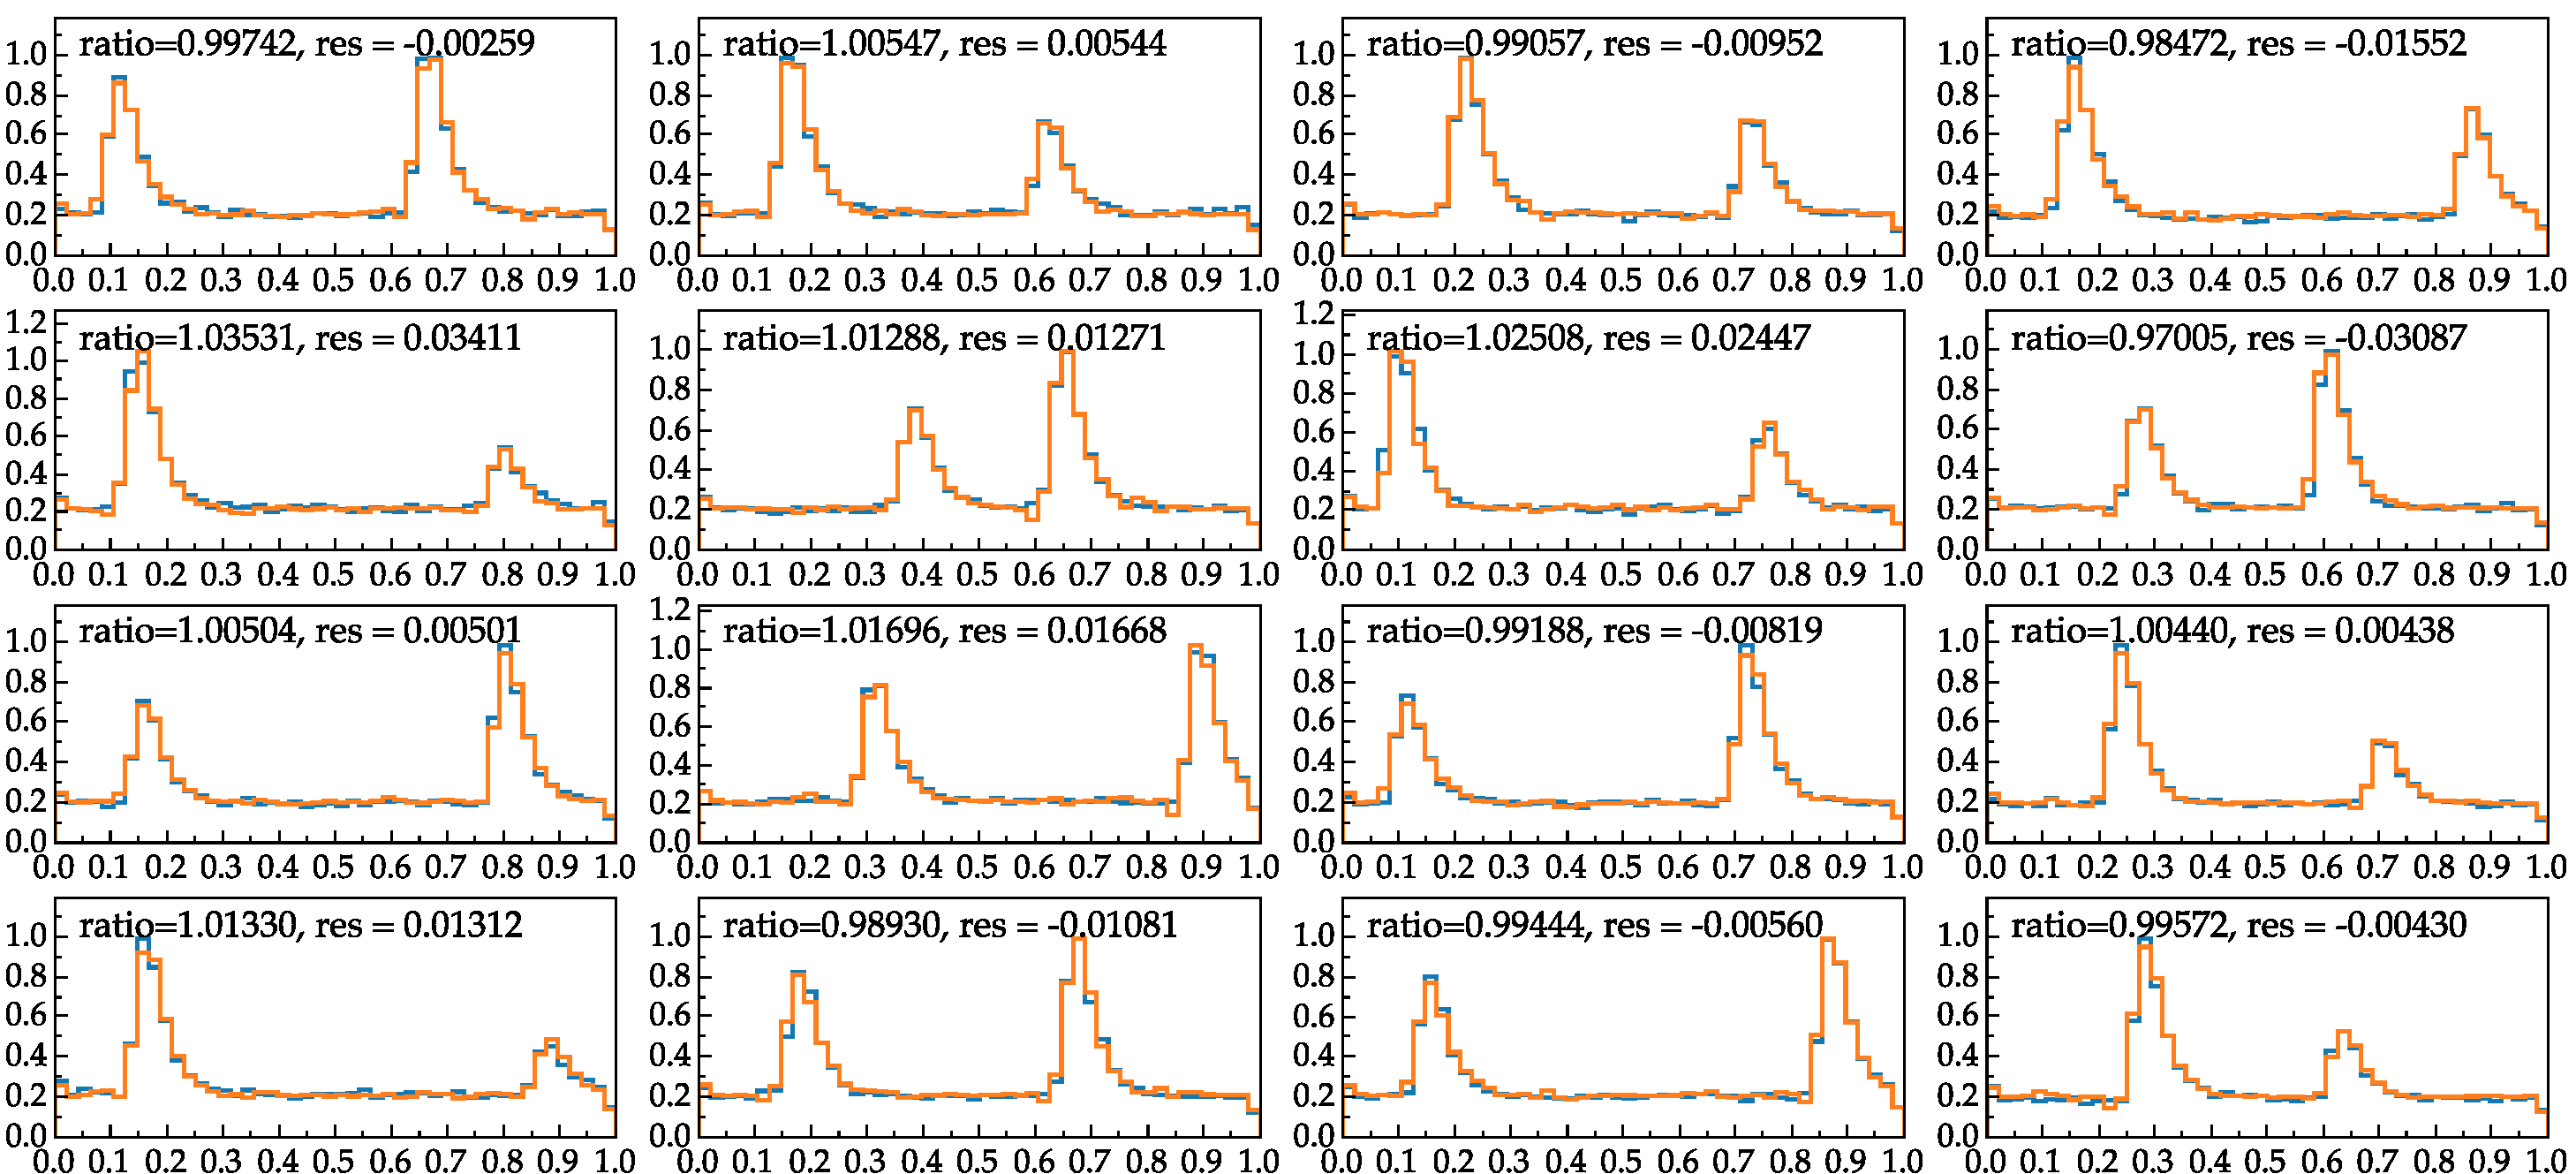
\includegraphics[width=0.9\columnwidth]{results_dp_96.pdf}
\caption{Generated double pulses plotted with the decompressed pulses overlayed. The compression is done with the improved auto-encoder [48,96,48,24,12,24,48.96,48] architecture. The data is produced by simulating a single pulse in the 48-bin region.} 
\label{fig:results_dp_96}
\end{figure}

The results show significant improvement in peak reconstruction from compressed latent space, where not only the peak positions are well reconstructed, but also the peak heights and withs have very close values to the original raw pulse. And the normalized difference of the peak integrals also shows significant improvements compared to the old network architecture and reaches a resolution of $1.4\%$.

\begin{figure}[h!]
\centering
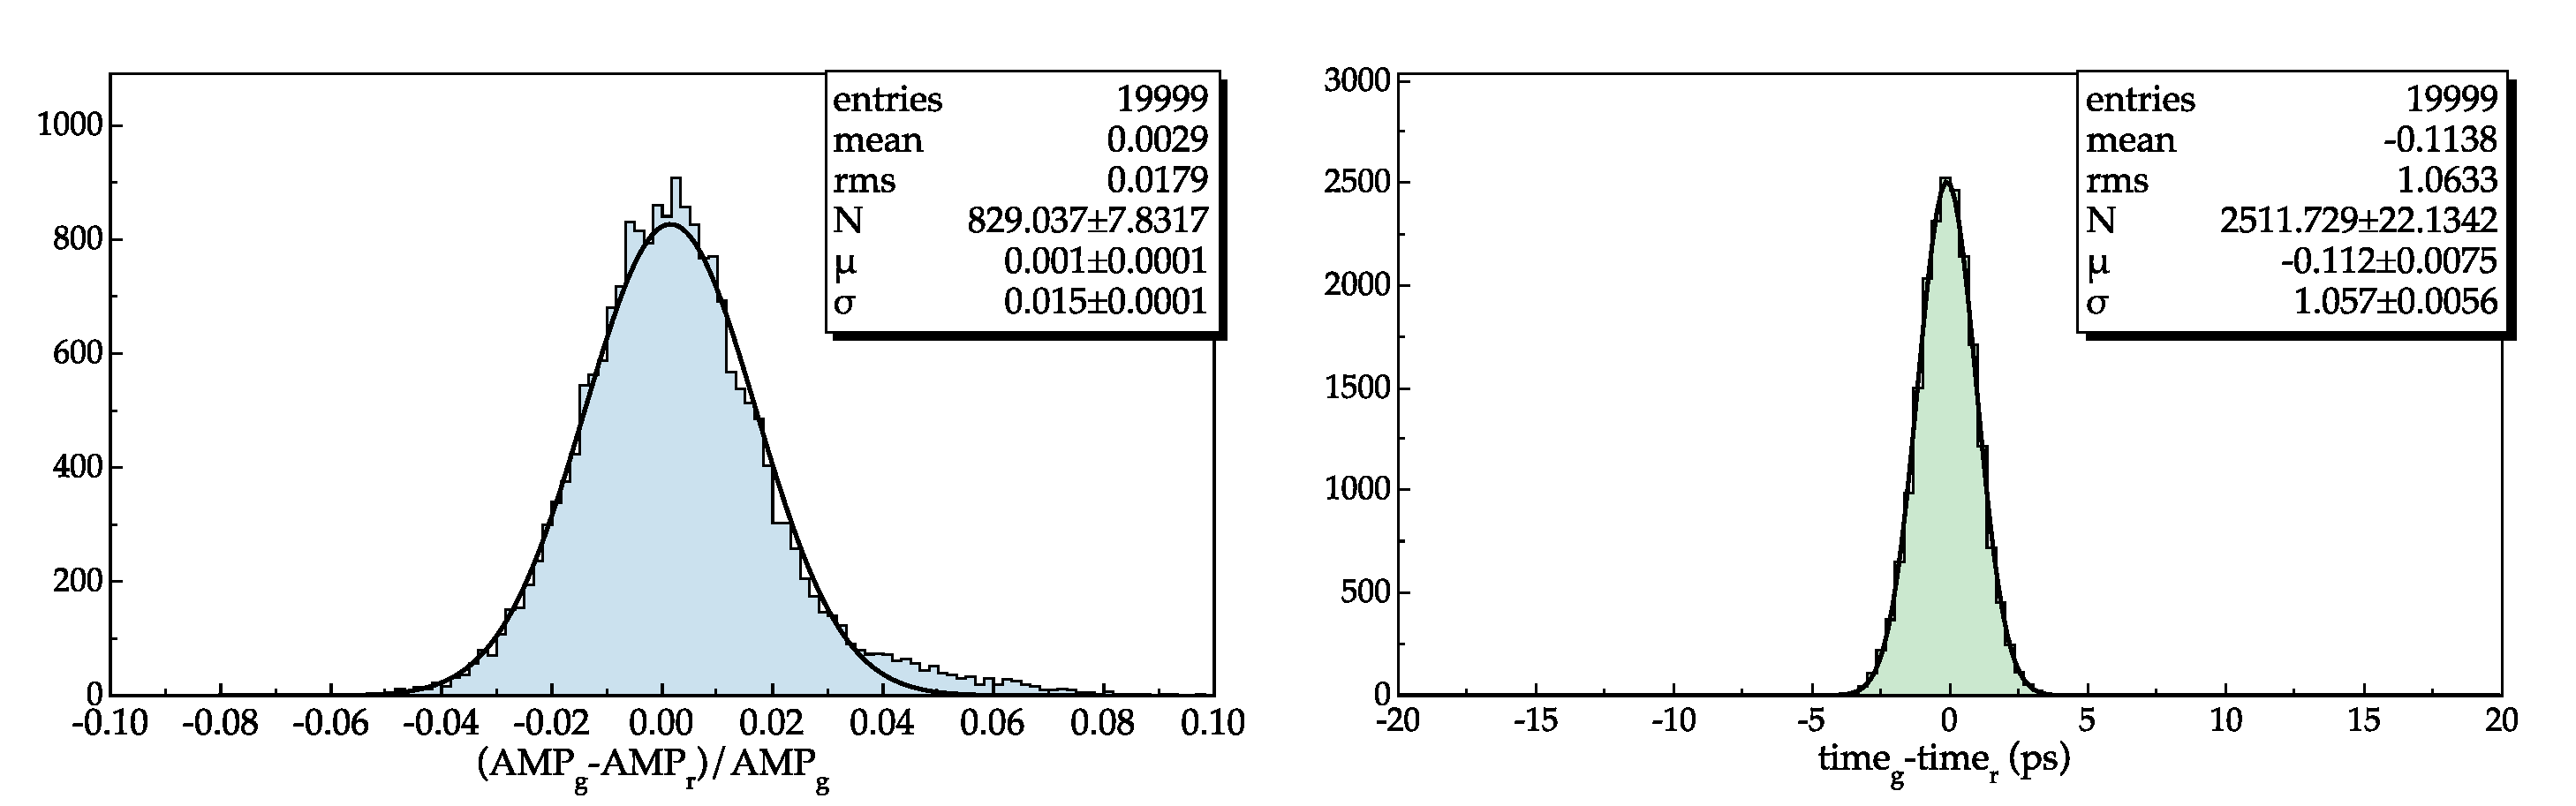
\includegraphics[width=0.9\columnwidth]{out_evaluate96_12_csv.pdf}
\caption{The resolution of the pulse integrals (double pulses). The integral of the pulse is compared to the integral calculated from decompressed (with network [48,96,48,24,12,24,48.96,48]) pulses (on the right), and the time calculated from the original pulse is compared to the time calculated from the decompressed pulse.} 
\label{fig:results_dp_96_res}
\end{figure}


\section{Studies with Experimental Data}

The neural network architecture tested on simulated data was used to train a neural network using real experimental data. As in our simulation studies, the pulses that are measured in one detector are very similar in width due to the same material with the same relaxation time and the same photo-multipliers with the same amplifiers. For our studies, we used pulse data from the Electromagnetic Calorimeter of CLAS12 detector, which makes up about $25\%$ of the data volume produced by CLAS12 data acquisition. 


\begin{figure}[h!]
\centering
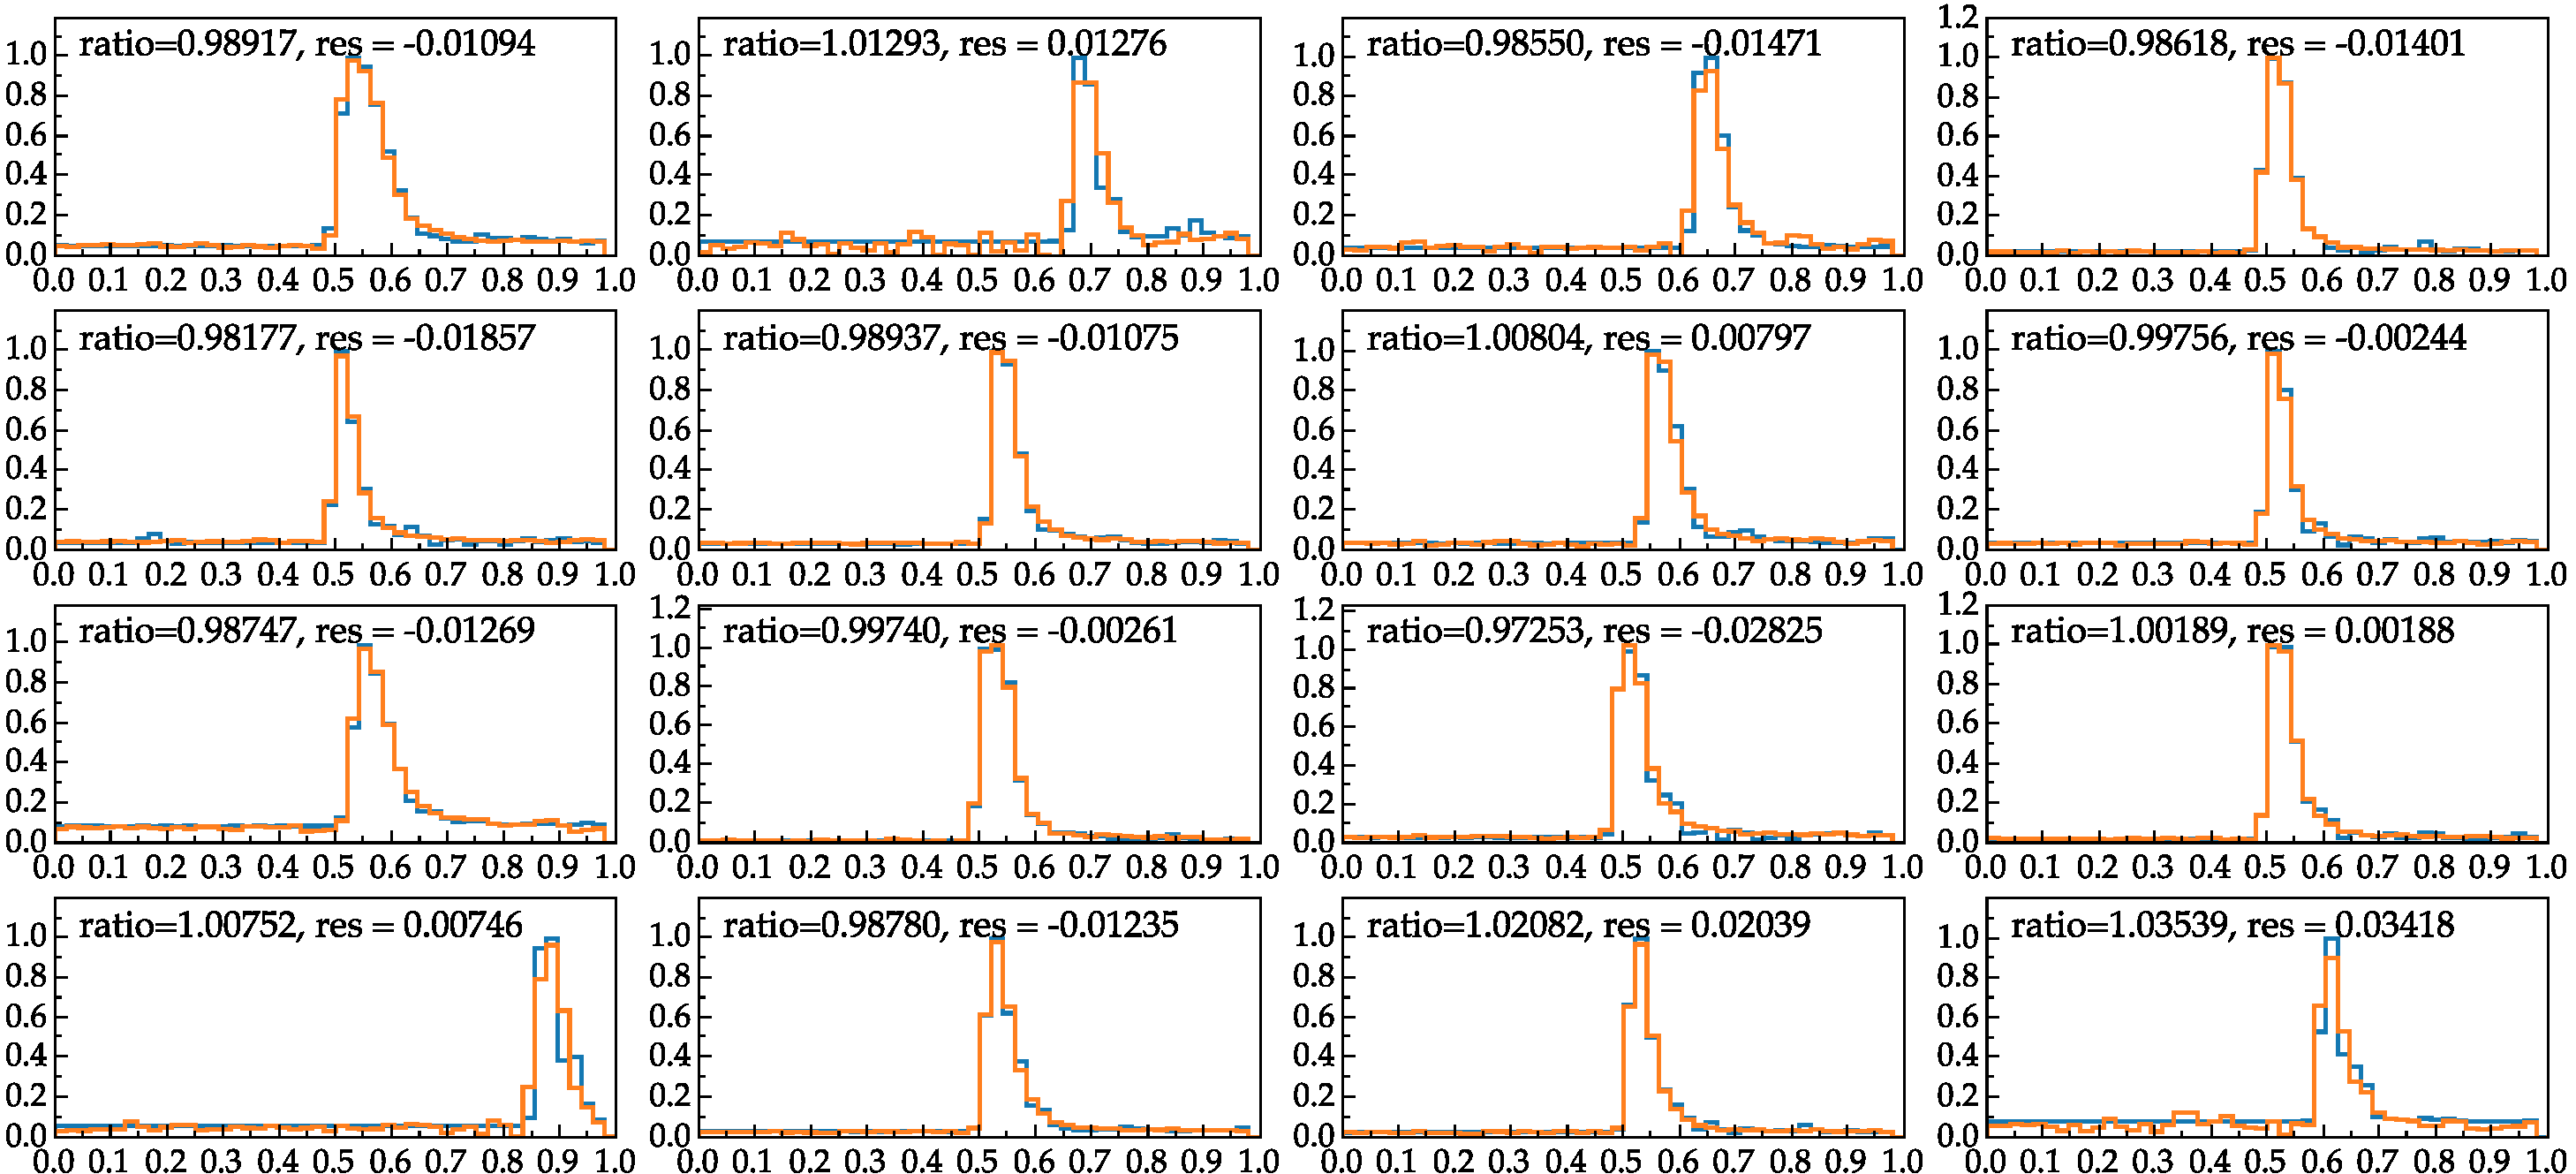
\includegraphics[width=0.95\columnwidth]{results_data_96.pdf}
\caption{Experimental data pulses plotted with the decompressed pulses overlayed. The compression is done with the improved auto-encoder [48,96,48,24,12,24,48.96,48] architecture. } 
\label{fig:results_data_96}
\end{figure}

\begin{figure}[h!]
\centering
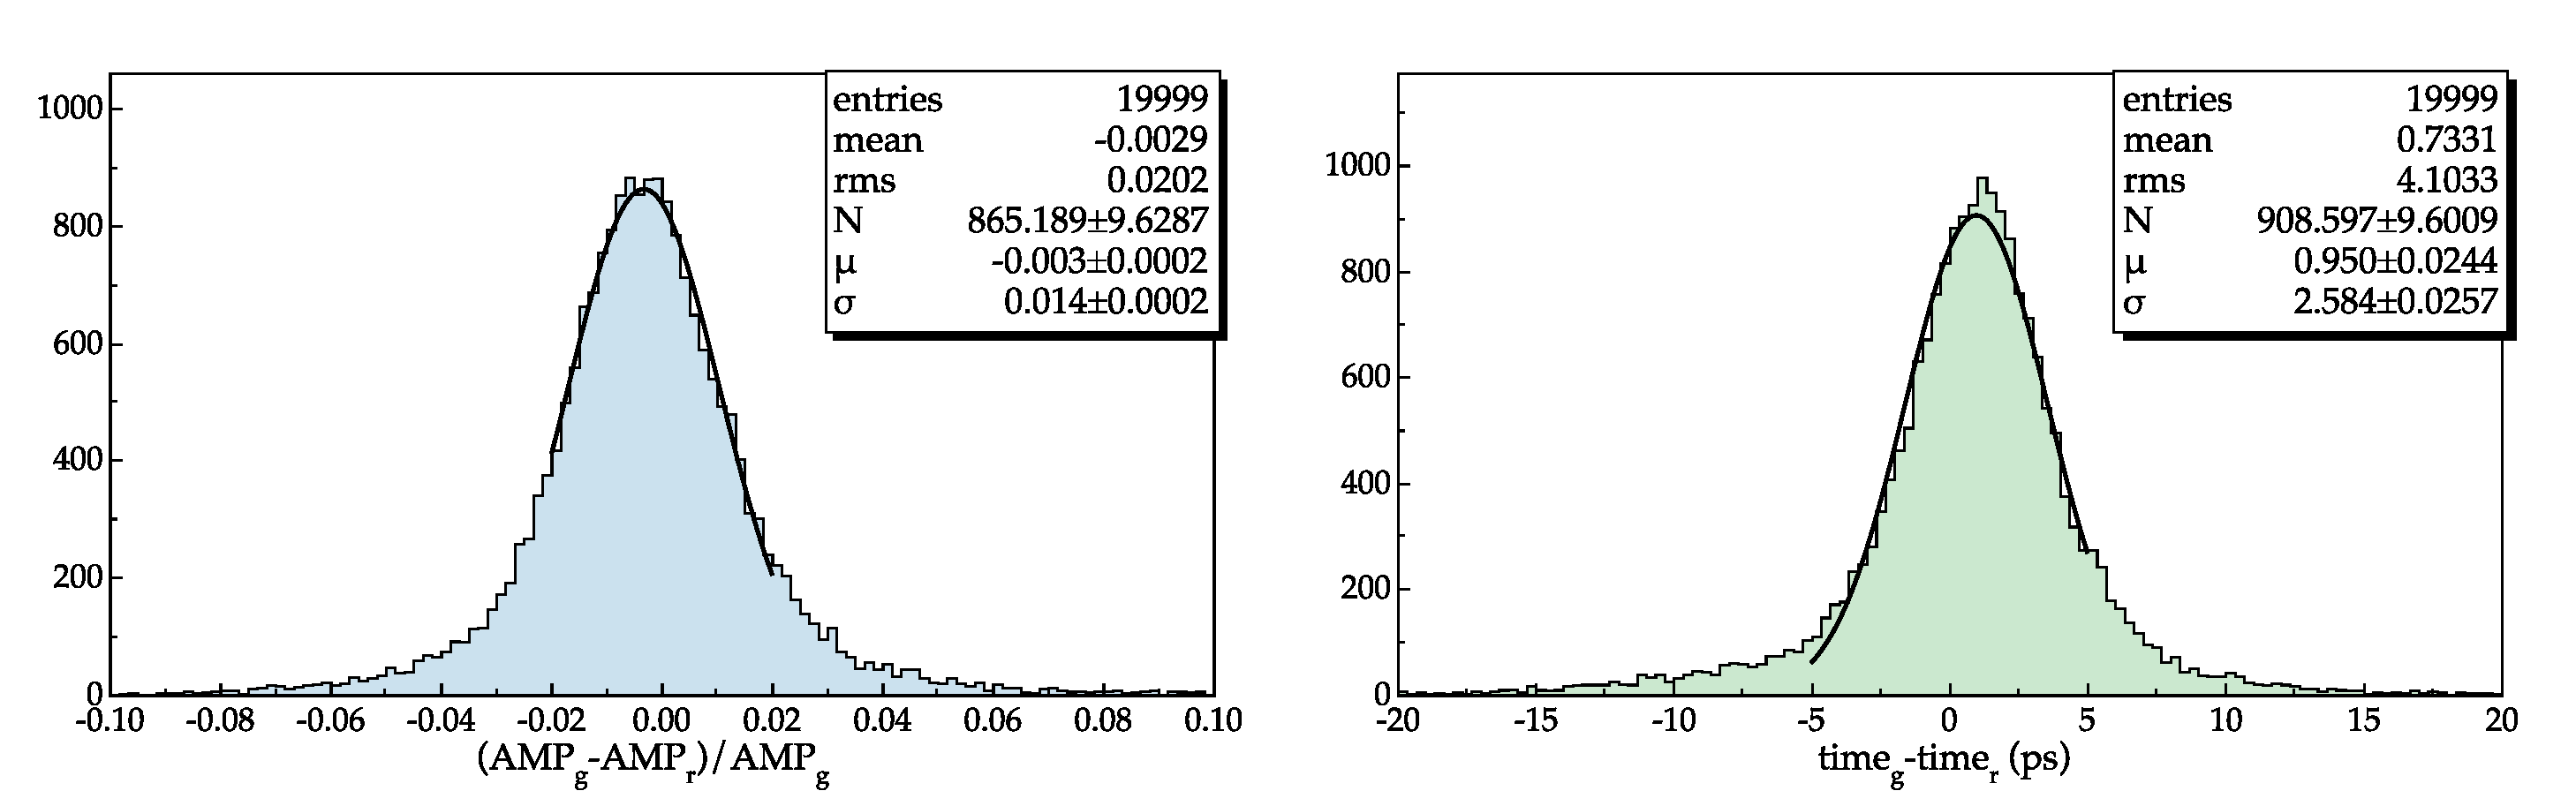
\includegraphics[width=0.9\columnwidth]{out_evaluate_csv_raw_96.pdf}
\caption{Resolution of the experimental pulses decompressed. Pulse amplitude resolution (on the left) and pulse timing resolution (on the right). } 
\label{fig:results_data_96_res}
\end{figure}


\section{Compression Factor Studies}

For studies in this article, we used compression factor 4, where the input data with 48 values was compressed into a latent space vector of length 12. However, the 
latent space vector can be changed to a smaller value to achieve a higher compression factor, but the resolution of the reconstructed pulse integral deteriorates as 
a function of the compression level. The following studies were done using a latent space layer set to 24, 8 and 6 lengths, increasing the compression ratio to 2, 6 and 8 respectively.

\begin{figure}[h!]
\centering
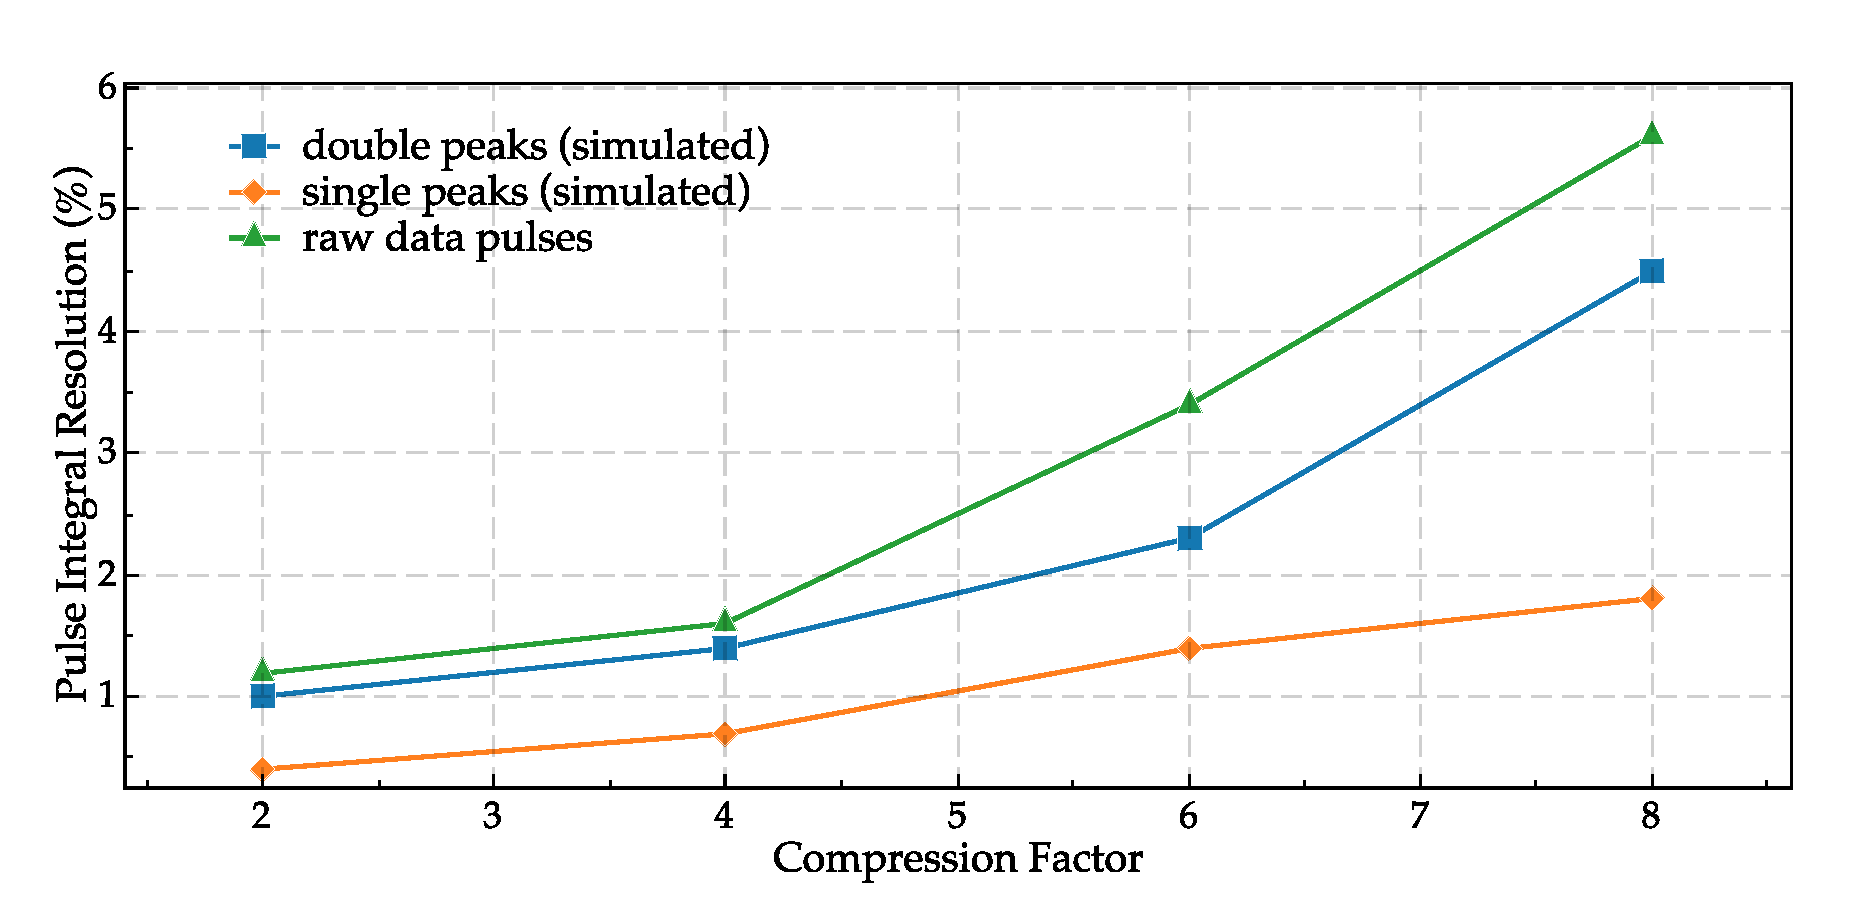
\includegraphics[width=0.95\columnwidth]{cfactor_summary.pdf}
\caption{The resolution of decompressed pulse integral as a function of compression factor.} 
\label{fig:compression_factor_summary}
\end{figure}

The result for three different data sets are shown in Figure~\ref{fig:compression_factor_summary}, the resolution decrease in single peak simulated data is linear and decreases with the increased compression ratio. In the double peak simulated and raw data the decoded peak resolution decreases rapidly with the compression ratio increase, reaching above $5\%$ for the compression ratio of 8.
The studied neural network (autoencoder) is capable of compression pulses into much smaller latent space and preserves very well the position of the peak but has some resolution depending on the compression ratio. Depending on the requirements of the situation different compression ratios can be used.

\section{Discussion}

So it goes.



\section{Acknowledgments}

This material is based upon work supported by the U.S. Department of Energy, Office of Science,
Office of Nuclear Physics under contract DE-AC05-06OR23177, and NSF grant no. CCF-1439079 and
the Richard T. Cheng Endowment. 
 
\bibliography{references}
\bibliographystyle{ieeetr}

\end{document}
